\subsection{De l'importance de composer les techniques de protection}

De plus en plus d'applications, en particulier
les applications web et les applications pour téléphone portable,
cherchent à utiliser le nuage, soit pour stocker du code ou des données, 
soit pour faire des calculs,
voir les deux à la fois.

En effet, le nuage peut offrir des services (que ce soit sous forme d'infrastructure,
de plateforme ou de logiciel) disposant d'une forte disponibilité et faciles à redimensionner.

Autrement dit, pouvoir utiliser le nuage est devenu un enjeu de la conception logicielle,
à cause des avantages de disponibilité et redimensionnement que cela offre.

Mais ce n'est pas le seul enjeux de la conception logicielle.

Vu que la plupart de ces applications manipulent des données personnelles, 
garantir la \emph{confidentialité} des données est également un enjeux de 
ces applications là; tout comme le sont les \emph{performances} pour garantir
une meilleure expérience à l'utilisateur de l'application.

Dans sa thèse, R. Cherrueau s'intéresse à trois techniques particulières
utilisées dans le développement logiciel et regarde comment elles interagissent
avec les trois enjeux cités plus haut.
Ces trois techniques, qu'on va décrire brièvement, sont
	le \emph{chiffrement},
	la \emph{fragmentation verticale} et
	l'\emph{exécution} de l'application \emph{chez l'utilisateur}.

\paragraph{Le chiffrement}
Lorsqu'il est bien utilisé, le chiffrement permet de garantir la confidentialité
des données de l'utilisateur.
De plus, dans certains cas, des calculs peuvent être faits sur les données chiffrées.
On appelle chiffrement homomorphe un chiffrement avec lequel on peut effectuer des calculs
avec les données chiffrées. Les chiffrement homomorphes totaux, comme celui de
Gentry (\textbf{référence à ajouter}) sont pour l'instant trop contraignants pour pouvoir être utilisés
dans la plupart des applications, mais les chiffrements homomorphes partiels,
c'est à dire les chiffrement avec lesquels on peut effectuer \emph{certaines}
opérations sur les données chiffrées, peuvent se révéler très utiles.
C'est le cas des chiffrements déterministes (dont les chiffrements symétriques)
qui sont des chiffrement homomorphes partiels, permettant le test d'égalité.

Dans tous les cas, le chiffrement implique un surcoût en terme de calculs,
donc diminue les performances. Dans certains cas, il améliore la confidentialité
et permet l'utilisation du nuage.

\paragraph{L'exécution côté client}
Si le programme était exécuté entièrement par la machine de l'utilisateur,
cela serait à la fois bon pour la confidentialité (car les données
ne seraient pas du tout exposées aux risques liés à l'utilisation du nuage
et du réseau) et pour les performances, puisque, à moins de traiter une 
trop grande quantité de données dans un calcul hautement parallélisable,
les performances du cloud sont moins bonnes que celles des machines des utilisateurs.
Par contre, l'exécution côté client ne permet pas de profiter des avantages du cloud.

\paragraph{La fragmentation verticale} consiste à séparer les différentes données
que manipule le programme entre deux clouds n'ayant aucun rapport entre eux
(à deux endroits géographiques différents, gérés par des entités différentes,
etc$\dots$).
Ceci permet de protéger celles des données personnelles qui sont constituées d'une
\emph{association} de deux données. Par exemple, dans une application stockant
un ensemble de rendez-vous, l'association $(\mathrm{date}, \mathrm{lieu})$
doit être protégée, car une personne malveillante ayant accès à ces deux
informations là à la fois pourrait suivre l'utilisateur de l'application.

La fragmentation verticale contribue à protéger la confidentialité,
mais d'une façon souvent moins forte que celles du chiffrement
ou de l'exécution côté client. Par contre, chacun des fragments
de données qu'elles génère peuvent être opérés séparément, en introduisant
ainsi, lorsque le programme le permet, une dose de parallélisation
supplémentaire qui peut améliorer les performances et permettre de tirer
encore plus d'avantages du nuage.

\begin{figure}
	\begin{center}
		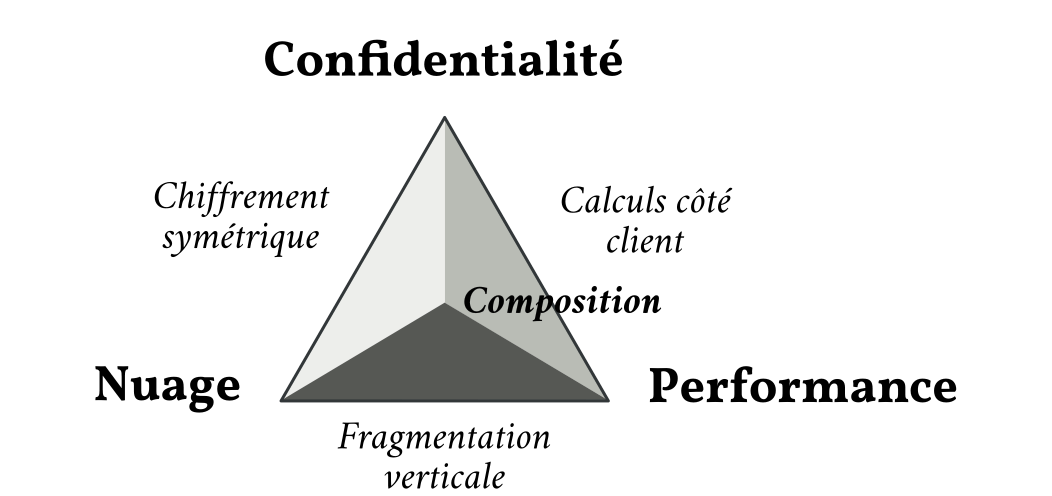
\includegraphics[width=0.7\textwidth]{snps.png}
		\caption{Enjeux et techniques dans le cloud-computing}
		\caption*{(image provenant de la thèse de Ronan Cherrueau)}
		\label{enjeux}
	\end{center}
\end{figure}

La figure \ref{enjeux} résume comment ces trois techniques
là interagissent avec les trois enjeux cités plus haut.

Dans sa thèse, Ronan Cherrueau montre qu'en composant ces différentes techniques
on peut à la fois profiter des avantages du nuage, protéger la confidentialité
et améliorer les performances d'un programme.

Pour pouvoir décrire comment s'effectue une telle composition,
pour pouvoir vérifier la correction d'une telle composition et
pour pouvoir raisonner dessus, Cherrueau a introduit un langage: C2QL.

\subsection{Un langage pour décrire la composition: C2QL}
Le langage C2QL donne une façon d'exprimer comment les techniques
mentionnées ci-dessus se composent avec les fonctions classiques de l'algèbre relationnelle.

Les données manipulées sont donc représentées sous forme de tables, ou relations,
c'est à dire un ensemble de lignes contenant des valeurs pour chacun(e) des 
différent(e)s attributs ou colonnes considéré(e)s.

Dans l'exemple de l'application stockant des rendez-vous, cette
table contiendrait autant de lignes que de rendez-vous stockés 
dans l'application et (par exemple) trois colonnes ou attributs: 
nom de l'utilisateur
ayant stocké le rendez-vous, date du rendez-vous et lieu du rendez-vous.

\paragraph{Les opérateurs empruntés à l'algèbre relationnelle}
présents dans ce langage sont
\begin{itemize}
	\item La projection, notée $\pi$
	qui consiste à ne considérer que certains des attributs de la table.
	\item La sélection, notée $\sigma$
	qui consiste, pour une table donnée, à ne considérer que
	les lignes sattisfiant un prédicat certain prédicat.
	\item 
\end{itemize}